\documentclass{article}
\usepackage[utf8]{inputenc}
\usepackage{amsmath}
\usepackage{flexisym}
\usepackage{graphicx}
\graphicspath{ {./images/} }
\usepackage[]{algorithm2e}
\usepackage{url}
\usepackage{enumitem}
\usepackage{listings}
\title{DV2574 - Assignment 2}
\author{Niklas Brännlund}
\date{March 2019}

\begin{document}
\maketitle

\section*{Problems}
    \section{Recurrent neural network (RNN)}

    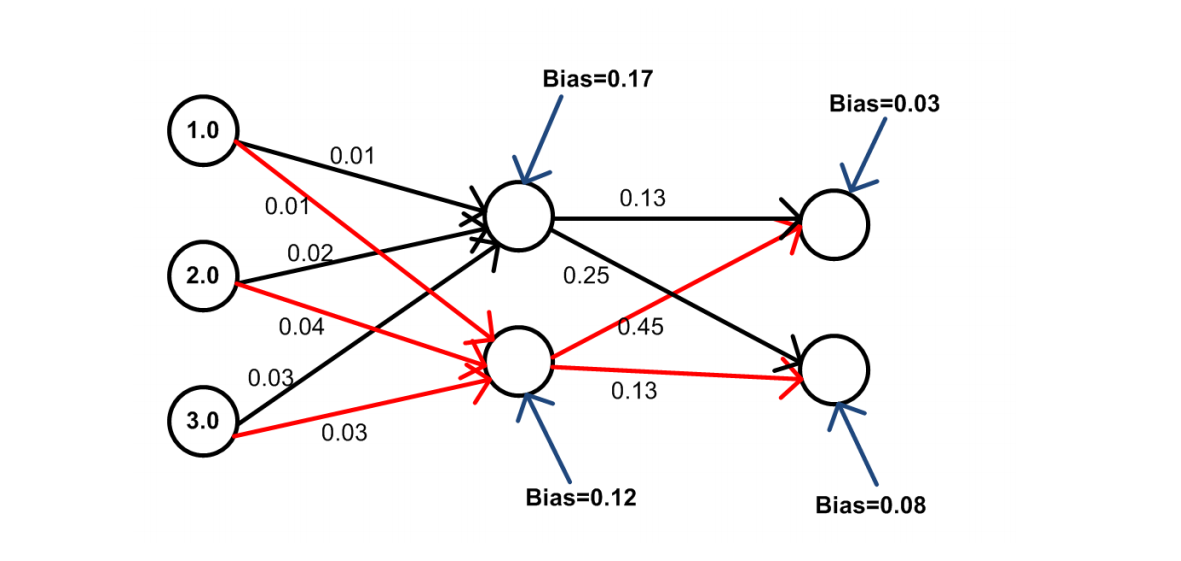
\includegraphics[width=\textwidth]{nn}
    Given the recurrent neural network above, we can conclude that it has the following properties:
    \begin{enumerate}[label=(\alph*)]
        \item 14 weights and biases
        \item 6 input-to-hidden weights
        \item 2 hidden node biases
        \item 4 hidden-to-output weights
        \item 2 output nodes 
        \item The input values of the network is 1,2,3
        \item Hidden node 1: $1*0.01 + 2*0.02 + 3*0.03 + 0.17 = 0.31 => \tanh(0.31)$, Hidden node 2: $1*0.01 + 2*0.04 + 3*0.03 + 0.12 = 0.3 => \tanh(0.3)$\\ Output node 1: $y_1 = \tanh(0.31) * 0.13 + \tanh(0.3)*0.45 + 0.03 = 0.200147$\\
        Output node 2: $y_2 = \tanh(0.31)*0.25 + \tanh(0.3)*0.13 + 0.08 = 0.192980$.\\ By using the Softmax function
        \begin{equation}
            S(y_i) = \frac{e^{y_i}}{\sum_j e^{y_j}}
        \end{equation}
        \begin{equation}
            S(y_1) = \frac{\exp{0.200147}}{\exp{0.200147} + \exp{0.192980}}
        \end{equation}
        \begin{equation}
            S(y_2) = \frac{\exp{0.192980}}{\exp{0.200147} + \exp{0.192980}}
        \end{equation}
        \item The values of the hidden nodes will be stored in two context nodes which sits below the hidden nodes. These will act as supplementary input for the hidden nodes in the next iteration  
    \end{enumerate}
    
    \section{Convolutional neural network (CNN)}
    
    
    This part is about constructing a two-input perceptron neural network model and using an algorithm for finding the final weights of the model. The inputs  $x_1$ and $x_2$ is described using the logical \textbf{OR} operator
    \begin{equation}
        \begin{tabular}{ | c | c | c | }
            \hline
            \multicolumn{2}{ |c| }{\textbf{Input variables}} & \textbf{OR} \\ 
            $\boldsymbol{x_1}$ & $\boldsymbol{x_2}$ & $\boldsymbol{x_1}$ $\cup$ $\boldsymbol{x_2}$ \\ \hline
            0 & 0 & 0\\
            0 & 1 & 1\\
            1 & 0 & 1\\
            1 & 1 & 1\\ \hline
        \end{tabular}
        \label{eq:or}
    \end{equation}
    Using the input from eq. \eqref{eq:or} in the following algorithm \\

    \begin{enumerate}
        \item Set initial weights $(w_1, w_2) = (0.5, 0.1)$ and bias $\theta = -0.1$. Learning rate $\alpha$ should be set to $\alpha = 0.01$ 
        \item Activate the model by applying inputs $x_1(p), x_2(p)$ and the output from the OR operator $Y_d(p)$ (which is the desired output). Calculate the actual output for iteration p=1 
        \begin{equation}
            Y(p) = step\Bigg[\sum_{i=1}^n x_i(p)w_i(p) - \theta\Bigg]
        \end{equation}
        where $step$ is a step function.
        \item Update the weights with the following equation
        \begin{equation}
            w_i(p+1) = w_i(p) + \Delta w_i(p)
        \end{equation}
        where $\Delta w_i(p)$ is the weight correction. It is defined as 
        \begin{equation}
            \Delta w_i(p) = \alpha\ x_i(p) e(p)
        \end{equation}
        where $e(p)$ is the difference between the desired output and the calculated result
        \begin{equation}
            e(p) = Y_d(p) - Y(p)
        \end{equation}
    \end{enumerate}
    By running the script \texttt{perceptron-neural-network.py} we get the output for the final weights to be
    $w_1=0.1$ and $w_2 = 0.5$.
    The algorithm logic for perceptron neural network can be found under \url{/algorithm/neuralnetwork.py}.
    \section{K means clustering}
    This section handles problem where k-means-algorithm is applied.
        \subsection{Image comparison}
        \label{im}
        Given two images \textbf{imA} and \textbf{imB} where each image is presented by by a 10x10 pixel matrix. Find out for which pixel coordinated there is a big difference in pixel values. This is done by first calculating a difference image \textbf{im}
        \begin{equation}
            \textbf{im} = |\textbf{imA} - \textbf{imB}|
        \end{equation}
        Given the difference image, we normalize this image with the following equation
        \begin{equation}
            \textbf{imNormalized} = \frac{\textbf{im} - im_{min}}{im_{max} - im_{min}}
        \end{equation}
        where $im_{min}$ and $im_{max}$ is the min and max value of \textbf{im}, respectively. Now we can apply K-means-clustering on \textbf{imNormalized} to obtain which pixels that have changed between \textbf{imA} and \textbf{imB}. The result is printed as a result matrix 
        
        \begin{equation}
            \textbf{imResult} = 
            \begin{bmatrix}
                0 & 0 & 0 & 0 & 0 & 0 & 0 & 0 & 0 & 0 \\
                0 & 0 & 0 & 0 & 0 & 0 & 0 & 0 & 0 & 0 \\
                0 & 0 & 0 & 0 & 0 & 0 & 0 & 0 & 0 & 0 \\
                0 & 0 & 0 & 0 & 0 & 0 & 0 & 0 & 0 & 0 \\
                0 & 0 & 0 & 0 & 0 & 0 & 0 & 0 & 1 & 1 \\
                0 & 0 & 0 & 0 & 0 & 0 & 0 & 0 & 1 & 1 \\
                0 & 0 & 0 & 0 & 0 & 0 & 0 & 0 & 1 & 1 \\
                1 & 1 & 1 & 1 & 1 & 1 & 1 & 1 & 1 & 1 \\
                1 & 1 & 1 & 1 & 1 & 1 & 1 & 1 & 1 & 1 \\
                1 & 1 & 1 & 1 & 1 & 1 & 1 & 1 & 1 & 1
            \end{bmatrix}
        \end{equation}
        where 1 stands for a significant change in pixel value and 0 is no significant change. This result can be reproduced by running the script \texttt{image-comparison.py}. The algorithm logic for k-means-clustering can be found under \url{/algorithm/kmeansclustering.py}.
        
        \subsection{Corrupted currency}
        Given a list of crypto currency prices that were gathered during a day. Use k-means clustering to find prices that were corrupted when they were stored. This problem uses the same algorithm as in section \ref{im}. Run the script \texttt{corrupted-currency.py} to get the result printed out. When using 6 clusters (setting NUM\_CLUSTERS = 6 in script) we get the following result
        
        \begin{enumerate}[label=(\alph*)]
            \item The corrupted prices were found to be 
            \begin{enumerate}
                \item 100587\$
                \item 101964\$
                \item 120967\$
            \end{enumerate}
            \item The max prices were found to be
            \begin{enumerate}
                \item 7845.0\$
                \item 7956.0\$
                \item 8215.0\$
                \item 8542.0\$
                \item 8150.0\$
                \item 8386.0\$
                \item 8219.0\$
                \item 7500.0\$
                \item 9257.0\$
                \item 8553.0\$
            \end{enumerate}
            \item the minimum prices were found to be
            \begin{enumerate}
	            \item 0.76\$
            	\item 0.78\$
            	\item 0.78\$
            	\item 0.72\$
            	\item 0.82\$
            	\item 0.82\$
            	\item 0.67\$
            	\item 0.72\$
            	\item 0.84\$
            \end{enumerate}
        \end{enumerate}
        We can see that one cluster is created where the values are above the max price of 20.000\$ and these are the prices that are to be seen as corrupt. When we use for example 4 clusters, we can still find the corrupted prices as they create an identical cluster as in the 6-cluster-case. Although, the min prices-cluster is different compared to when using 6 clusters. This can be seen when running the script by setting the NUM\_CLUSTERS variable to 4.
\end{document}
